\documentclass[12pt]{article}

% --------------------
% Basic Packages
% --------------------
\usepackage[a4paper,margin=1in]{geometry}
\usepackage{setspace}
\usepackage{graphicx}
\usepackage{amsmath}
\usepackage{amssymb}
\usepackage{array}
\usepackage{float}



\onehalfspacing

% --------------------
% Title and Author
% --------------------
\title{QoS-Aware Routing Techniques for Multimedia
Transmission in Wireless Networks}
\author{Beerala Dinesh}
\date{}

\begin{document}
	\maketitle
	
	\section{Introduction}
	Quality of Service (QoS) aware routing\cite{Goyal2023} is a critical requirement for multimedia communication in wireless networks because multimedia communication is very sensitive to delay, jitter, packet loss, and bandwidth changes. Unlike in the case of data communication, in multimedia communication, a guaranteed level of quality of service should be ensured for the purpose of smooth communication, video quality, etc. The problem of ensuring quality of service in wireless networks is further complicated by the movement of nodes in wireless networks, fading, interference, medium contention, and the battery power of nodes, which changes very rapidly in wireless networks. Therefore, the above-mentioned problems of wireless networks can be addressed through quality of service aware routing solutions. The routes in these solutions ensure the quality of service requirements of the application. These routes are determined based on a combination of metrics. This assignment describes some of the quality of service aware routing solutions and their application in multimedia communication in different wireless networks
    QoS-aware routing is, at its core, a matter of deciding what's important for a particular app and making that clear. So, a protocol that doggedly tries to minimize delay might add a lot of control overhead, which consumes bandwidth that could have been available for the multimedia stream itself. It might also prioritize reliability with multipath forwarding, which could improve delivery but at the cost of increased jitter because those paths don't necessarily share a similar delay profile. In sensor and IoT-related cases, energy is also an important consideration because continuous signaling, retransmission, and processing exhaust nodes that operate on batteries and reduce the useful lifespan of a network. Because these priorities vary depending on the case, QoS-aware routing approaches vary depending on whether the network is a multimedia sensor network, a mobile ad-hoc network, an IoT network for smart cities, a heterogeneous wireless network, or a software-defined network.
    QoS-based routing exists because of one simple fact: multimedia traffic is not homogeneous, even in an individual flow. For example, interactive voice and video calls require extremely small delays and no jitter at all. A one-way video feed may be able to tolerate a slightly larger delay, but it has extreme sensitivity to repeated packet loss or sudden degradation in bandwidth. And in a wireless network, there are always background flows sharing the same spectrum. As a result, competition from other flows can quickly consume all available service in a wireless network. The key to understanding this is to realize how important it is to understand these behaviors if we are to fairly evaluate various routing techniques. A routing algorithm may perform well on average, but fail in practice if it cannot deal with sudden changes in delay, loss, or competition.
    \subsection{Motivation: Multimedia QoS requirements in wireless networks}
    For multimedia communication like video streaming, video conferences, and interactive audio communication, performance guarantee is required for the purpose of providing quality of service to the end user. The quality of service provided to the end user of a wireless network is highly dependent on the end-to-end delay, jitter, packet loss, and throughput provided to the end user, as even a slight change in the values of these parameters will cause desynchronization of the audio and video being sent out or the actual video being received by the end user. Unlike other forms of communication, multimedia communication requires the association of an implicit deadline with the communication. The late arrival of a packet is considered equivalent to the loss of a packet. The wireless medium has introduced many complexities to the communication that takes place on the wireless medium.


	\section{Background and Conceptual Foundations}
	The motivation behind \cite{Chiwariro2022789,Sen2010CrossLayerSurvey}the implementation of Quality of Service aware routing in wireless networks for multimedia applications comes from the premise that the network not only offers connectivity but also offers some kind of quality. This means that the application of multimedia, being highly sensitive to the quality of the data being sent over the network, should be taken into consideration in the routing protocol using the quality of the data in terms of delay, jitter, bandwidth, and loss probability instead of hop count. In wireless multimedia sensor networks, these factors have to be combined with the scarce resources available to the nodes, such as the battery energy available to the nodes, the limited processing power of the nodes, and the unstable wireless communication links due to interference effects. This section reviews the premise established in the literature for reasoning about wireless multimedia sensor networks, including the differences between network QoS and user QoS, application QoS to routing metrics, as well as the effects of mobility, channel variations, and medium access contention. This section integrates these premises with the established survey views of wireless multimedia sensor networks and multi-channel wireless sensor networking.
    \subsection{QoS and QoE metrics for multimedia transmission}
    QoS \cite{9074932}is a set of network parameters that directly affect the delivery of multimedia content, while QoE is the user’s perception of the received multimedia content in terms of the audio or video received. In the context of routing in multimedia networks, the QoS parameters are generally the end-to-end delay, delay variation or jitter, packet delivery ratio or loss rate, throughput or bandwidth provided, and sometimes the route or link stability. These parameters are affected by the multimedia session established due to the delay associated with multimedia packets received after a certain period of time, which is similar to the packets lost in the network. Therefore, the QoE is a function of the QoS provided by the network. In terms of the routing process for multimedia content, the routing process is a function of the constraints and objectives set for the process. These constraints and objectives are the basis for the routing process and have been emphasized in the foundational papers on wireless multimedia sensor networks and multi-channel wireless sensor networks.
    \begin{table}[htbp]
	\centering
	\caption{QoS and QoE-related metrics commonly used in multimedia-aware routing and their practical interpretation (compiled from \cite{Goyal2023,Chiwariro2022789,9074932})}
	\label{tab:qos_metrics_multimedia}
	\renewcommand{\arraystretch}{1.2}
	\resizebox{\textwidth}{!}{%
	\begin{tabular}{|p{3.2cm}|p{5.2cm}|p{7.2cm}|}
		\hline
		\textbf{Metric} & \textbf{What it measures} & \textbf{Why it matters for multimedia} \\
		\hline
		End-to-end delay & Total time from source to receiver & High delay increases buffering and harms interactivity in calls and gaming \\
		\hline
		Jitter & Variation in packet delay over time & High jitter causes playback instability and forces larger buffers \\
		\hline
		Packet loss rate & Fraction of packets that do not arrive & Loss creates video artifacts, audio dropouts, and decoding failures \\
		\hline
		Packet delivery ratio & Fraction of packets successfully delivered & Low delivery ratio reduces visual continuity and audio reliability \\
		\hline
		Throughput & Achieved data rate at the receiver & Insufficient throughput prevents sustaining target bitrate and causes stalls \\
		\hline
		Available bandwidth & Estimated spare capacity along a path & Used to decide whether a path can carry a stream without persistent congestion \\
		\hline
		Link quality indicator & Signal or error-related estimate of link reliability & Helps avoid unstable links that trigger retransmissions and delay spikes \\
		\hline
		Route stability & Expected lifetime of a chosen route & Short-lived routes increase re-routing events and disrupt streaming continuity \\
		\hline
		Control overhead & Extra routing/control traffic generated & Excess overhead consumes capacity needed for media packets and increases contention \\
		\hline
		Energy consumption & Battery usage due to forwarding and control & In WSN/IoT, energy drain shortens network lifetime and service continuity \\
		\hline
		QoE proxy (e.g., PSNR) & Media quality estimate derived from received video & Captures perceptual impact beyond raw network metrics and guides QoE-aware routing \\
		\hline
	\end{tabular}}
\end{table}
\begin{figure}[htbp]
	\centering
	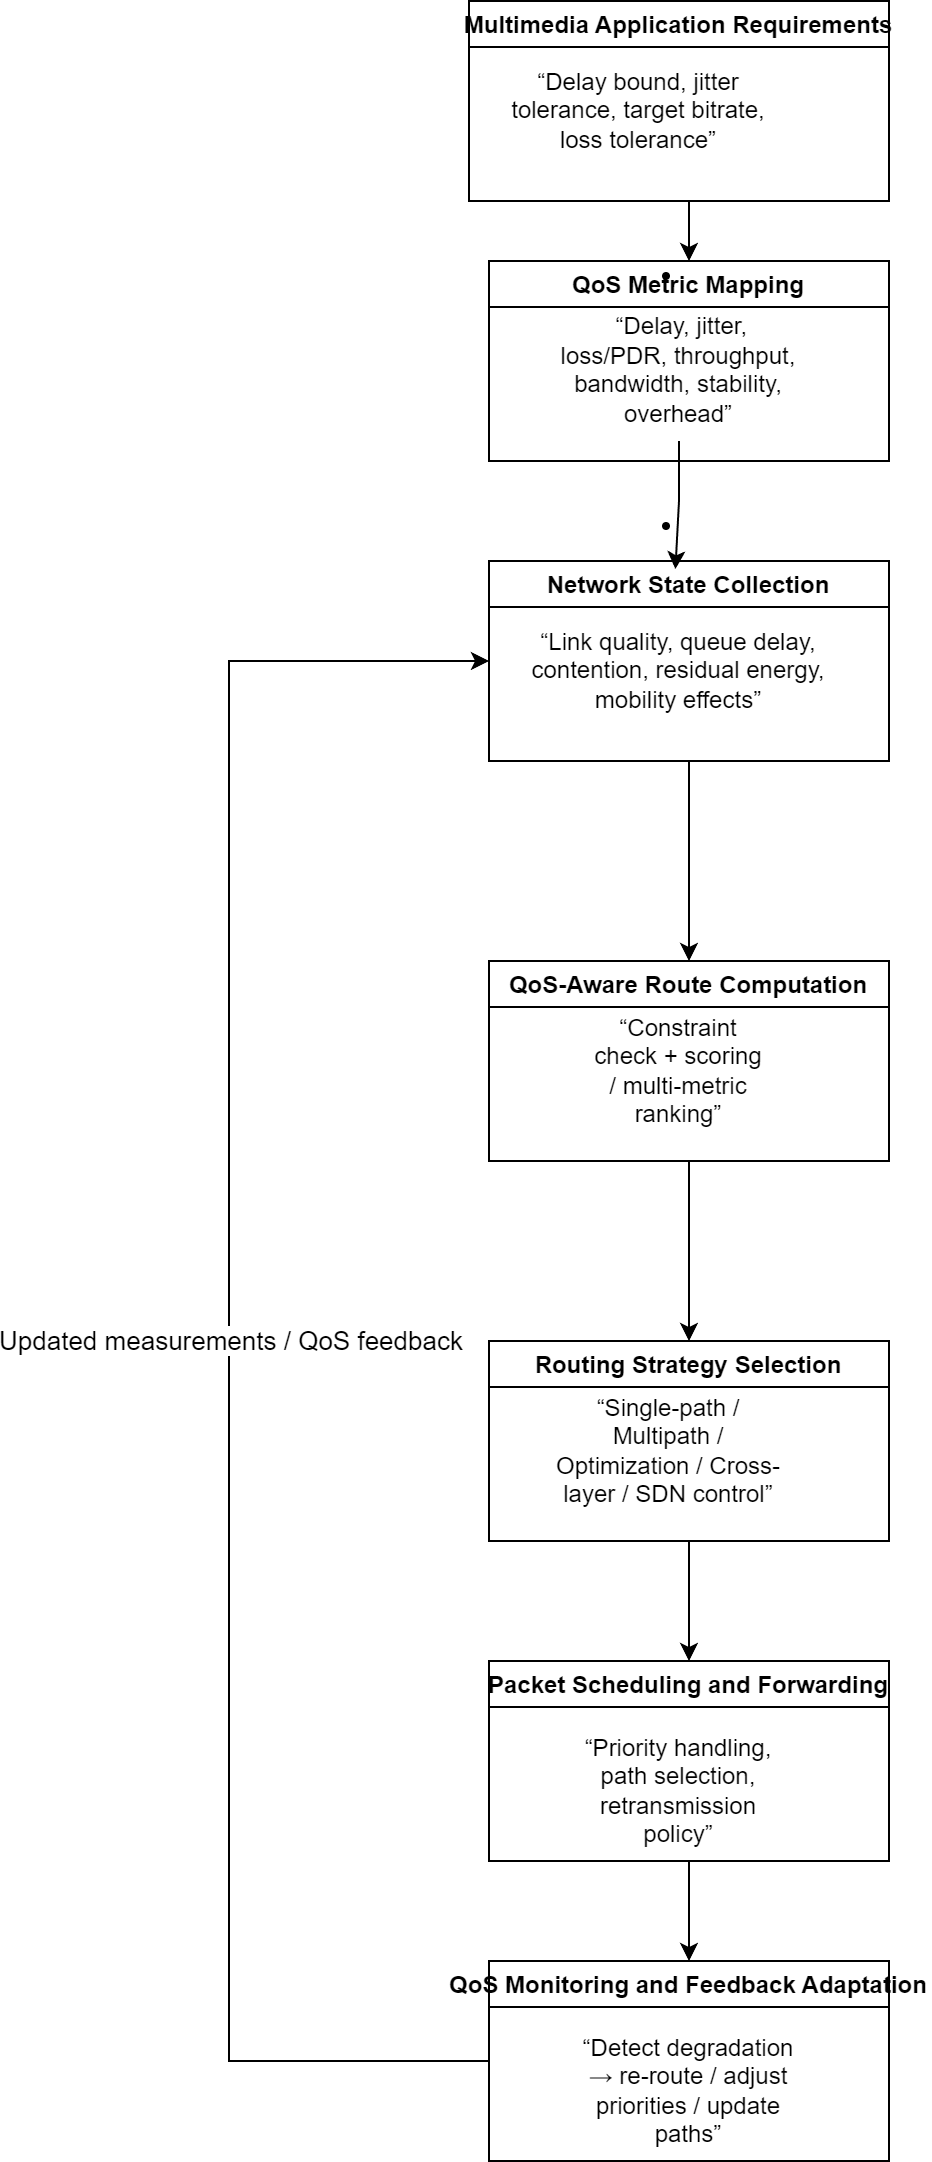
\includegraphics[height=0.94\textwidth]{fig_qos_pipeline_vertical.png}
	\caption{Vertical pipeline view of QoS-aware multimedia routing, showing requirement mapping, state collection, route computation, forwarding, and feedback-based adaptation (summary based on \cite{Chiwariro2022789,Goyal2023,Goyal2025321}).}
	\label{fig:qos_pipeline_vertical}
\end{figure}

    \subsection{Wireless multimedia network types and traffic characteristics}
    Wireless multimedia delivery is also present within other families of networks that are associated with this particular network type. All of the above network types have their own presumptions that affect the routing process. Wireless multimedia sensor networks are a class of networks that are primarily focused on the delivery of multimedia information such as images and videos, which are usually sent from more than one source to one or more sink nodes. It is a network type that has a lot of issues associated with it. The presence of an option to transport the data through more than one channel within a wireless sensor network gives rise to a multi-channel wireless sensor network that has an associated cost. The conceptual implications of this particular statement is that an optimal route is one that has an associated cost as well as enough capacity and stability of conditions of contention over a particular period of time. The metrics that are dominant within the routing process are usually dependent on the particular network type. The cost has to be updated frequently.
    \subsection{QoS routing formulation and design dimensions}
    QoS-aware routing can be described as "the process of finding a route or a set of routes that satisfy a given set of constraints while optimizing a given objective." The basic forms of QoS-aware routing are single constraint routing, multiple constraint routing, and optimization of multiple objectives. The last two forms include delay minimization and energy minimization. The above background also describes the role of design factors used in QoS-aware routing. What metrics are used to define what is seen in QoS-aware routing? Is it delay measurements, bandwidth estimates, link quality, or a combination of everything? How are constraints handled in QoS-aware routing? Is there admission control, route feasibility, or soft constraint ranking when hard constraints are present? How are routes maintained? How does QoS-aware routing handle changes in the environment? Is there periodic maintenance or event-driven maintenance? There is also overhead management, which is an important factor used in QoS-aware routing. The QoS states used can cause significant overhead, thereby degrading the performance of wireless multimedia networks. All the above background leads to the next section.
	\begin{table}[htbp]
	\centering
	\caption{Comparison of representative QoS-aware routing approaches for multimedia transmission across wireless network contexts (compiled from \cite{Chiwariro2022789,Goyal2023,Jara20211,Suseela20201248,Suguna2022,Srinivasulu2023,Karunkuzhali202517951,Singal2022,9939088})}
	\label{tab:comparison_qos_routing}
	\renewcommand{\arraystretch}{1.2}
	\resizebox{\textwidth}{!}{%
	\begin{tabular}{|p{3.1cm}|p{4.6cm}|p{4.2cm}|p{6.9cm}|}
		\hline
		\textbf{Network context} & \textbf{Representative approach} & \textbf{Main QoS focus} & \textbf{Typical limitations} \\
		\hline
		WMSN multimedia sensing & Surveyed QoS routing families & Delay, loss, energy & Hard guarantees under interference and resource scarcity \\
		\hline
		Heterogeneous MANET video & Surveyed QoS methods & Delay, jitter, robustness & Mobility-driven instability and fluctuating capacity \\
		\hline
		MANET video streaming & Multimetric and social-aware routing & QoS with trust-aware forwarding & Metric collection overhead and sensitivity to mobility and partitions \\
		\hline
		WMSN multipath delivery & Priority-based multipath optimization & Reliability, throughput, delay stability & Higher state maintenance and risk of inter-path contention \\
		\hline
		IoT multipath routing & Energy-efficient multipath with hybrid optimization & Energy, lifetime, latency & Computation and signaling overhead from optimization and clustering \\
		\hline
		Software-defined multimedia & Latency-aware controller-based routing & Low latency for interactive flows & Controller responsiveness limits and dependence on global state accuracy \\
		\hline
		Edge ad hoc multicast & QoS-aware mesh-based multicast concepts & Group efficiency and robustness & Membership maintenance complexity and multicast control overhead \\
		\hline
		SDN QoS multipath & QoS-aware multipath traffic engineering & Bandwidth and delay control & Control-plane overhead and scalability constraints under frequent changes \\
		\hline
		IoT smart-city WSN & QoS-aware routing for data collection & Latency, energy, security & Scalability issues with dense nodes and variable link quality \\
		\hline
	\end{tabular}}
\end{table}
\begin{figure}[H]
	\centering
	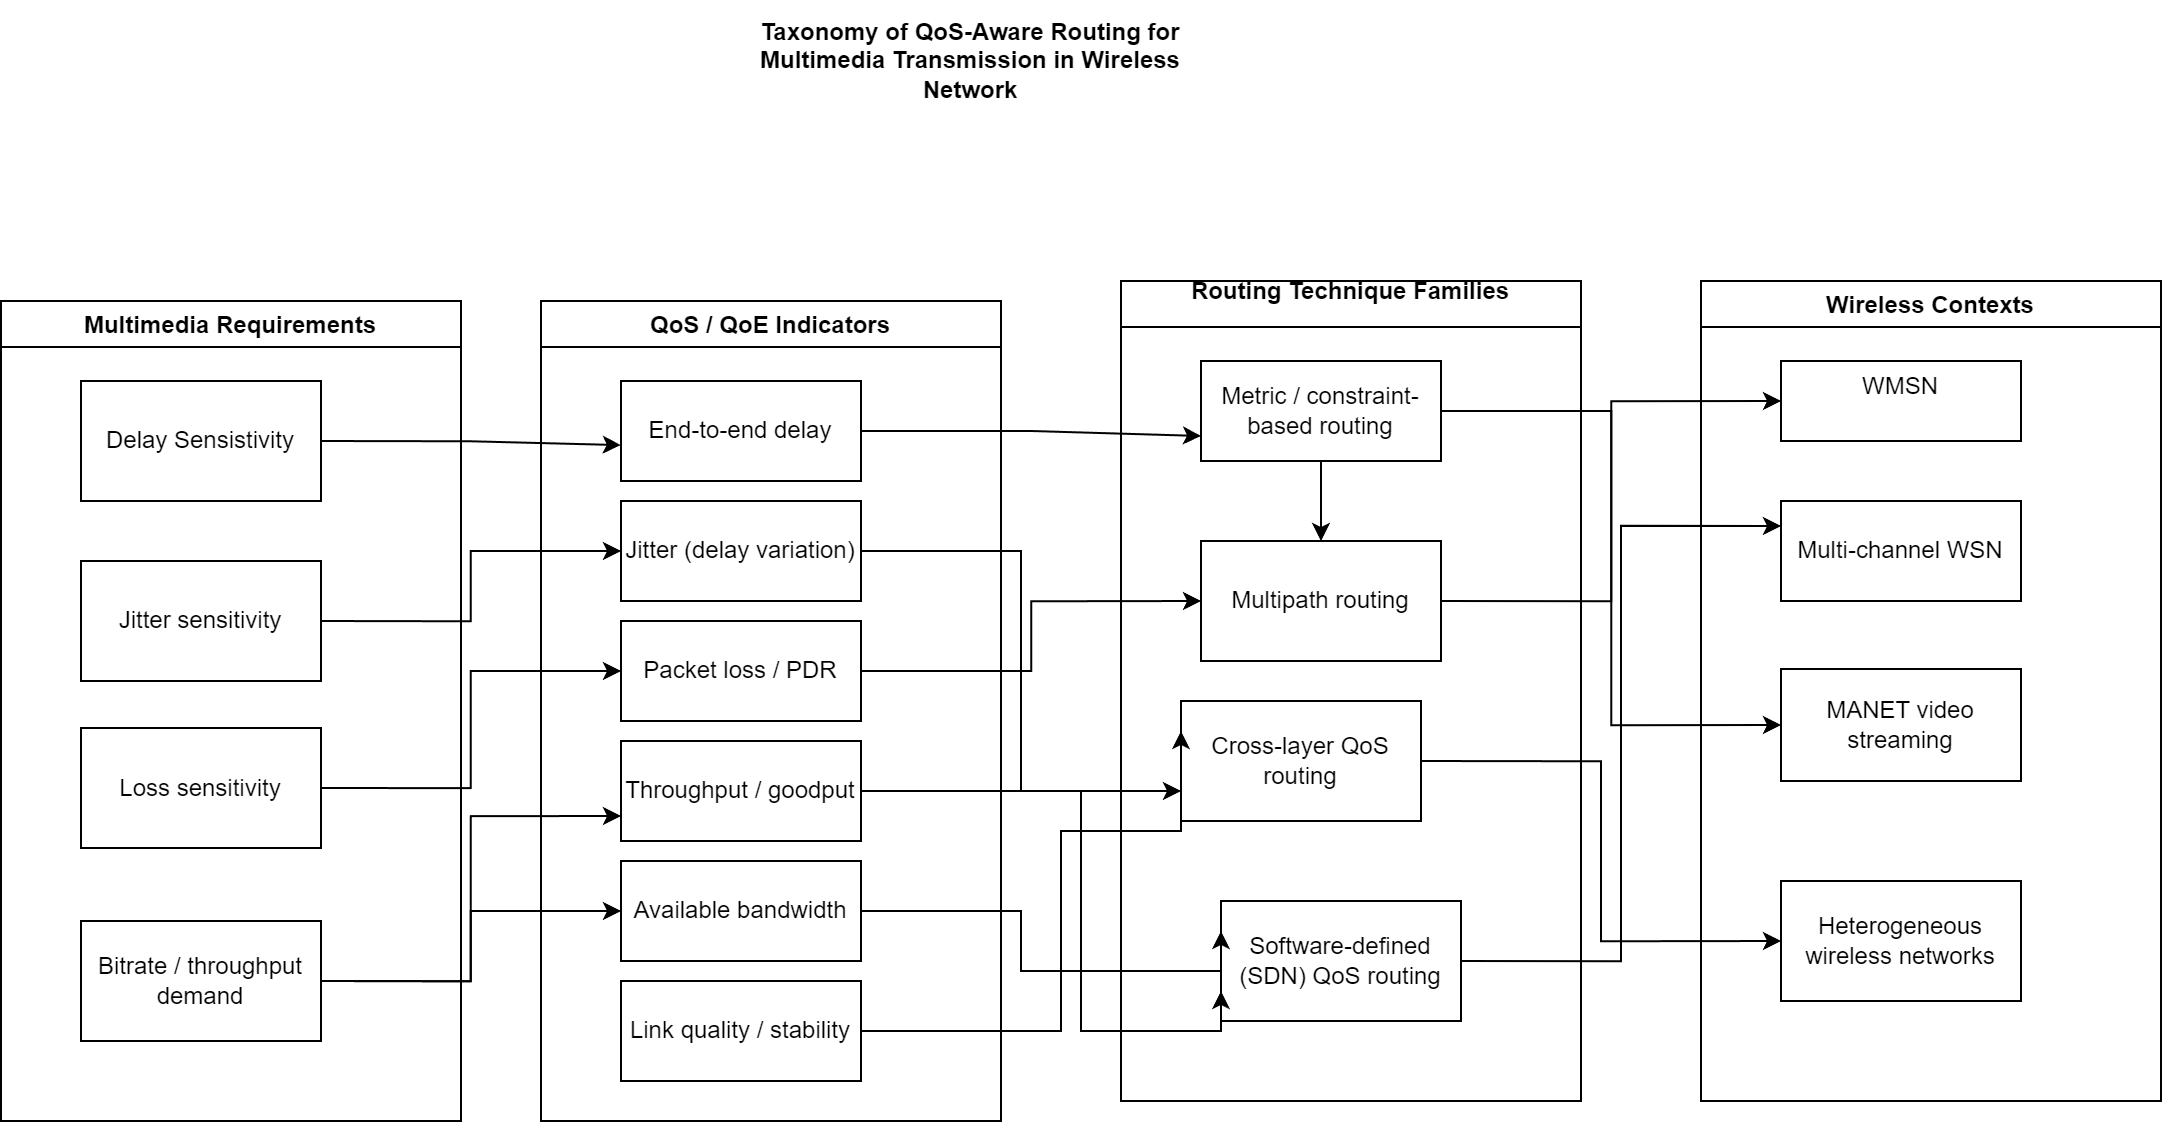
\includegraphics[width=0.85\textwidth]{fig_taxonomy.png}
	\caption{Taxonomy of QoS-aware routing for multimedia transmission in wireless networks (summary based on \cite{Chiwariro2022789,Goyal2023,Benmansour2021,9074932}).}
	\label{fig:qos_taxonomy}
\end{figure}
\subsection{Multi-channel effects on QoS-aware routing}
The multi-channel mode of operation also changes the routing issue since the quality of a given route is determined not just by the nodes traversed, but also the channels used along the way. The use of different channels can help reduce interference, thereby increasing overall system capacity, an issue of significant importance to multimedia applications that demand high throughput rates. However, the selection of appropriate channels also raises new issues of contention since neighboring routes may interfere with each other, even if different channels are used, owing to hardware capabilities, partial overlap of channels, as well as switching delays between channels. The routing metric may need to be extended to include new information, like expected contention per channel, switching delays, as well as the probability of collisions given the local traffic load. The issue of multi-channel wireless networks is perhaps best illustrated with regard to wireless sensor networks, where multimedia packets need to be transmitted with appropriate delay, given the capabilities of sensor nodes.

	

	\section{Core Concepts and Approaches}
    The mechanisms \cite{Fan2019CrossLayerLyapunov}through which QoS-conscious routing does its business in multimedia communication are similar to a collection of approaches, which consider what the service requires when it is being routed. Routing in multimedia communication based on QoS has approaches in which the service requirements are taken into account when carrying out routing. Such qoS- routing approaches are significant, in case of multimedia communication. Multimedia does not make much sense on the normal path of packet routing. The reason is the fact that it does not discriminate between packets. On the hand QoS-aware routing techniques adopt decisions, which are more multimedia-friendly. Multimedia requires that things work. These are assured delay, acceptable jitter but not excessive throughput as well as acceptable loss rates. Network issues are also aware of network problems with QoS-aware routing methods. These issues consist of time varying channels of change, mobility and energy restrictions. These are the things that QoS-aware routing methods take into consideration in their choices. They attempt to ensure that multimedia can work in wireless networks. It is crucial, as QoS- routing techniques since they are interested in ensuring that individuals are able to utilize multimedia without issues.
	\subsection{Metric-based and constraint-aware QoS routing}
    A primary approach\cite{Karunkuzhali202517951,Jara20211,Goyal2025321} to QoS-based routing is to express QoS requirements as specific constraints and multi-metric decision functions. In this approach to QoS-based routing protocol design, a routing protocol typically employs a set of metrics, such as delay, residual capacity, route stability, and link quality, to select a route that fulfills certain feasibility constraints or optimizes a composite metric score. Multimedia video streaming is a prominent application of multi-metric routing in mobile ad-hoc networks because of the dynamic nature of route quality, which can change rapidly due to mobility. Moreover, a route that is optimized for hop count may cause high jitter and loss. For IoT-based routing, this is extended to accommodate other service requirements of smart cities.
    \subsection{Multipath QoS routing for multimedia reliability}
    Normally, multipath routing \cite{Suseela20201248,Suguna2022,Srinivasulu2023,Abazeed2019CLMR} is used in multimedia communication due to its ability to improve communication robustness in the event of failure of the links, as well as its ability to improve load distribution even in the event that the rate requirements cannot be supported by a single path. The basic principle that is used to improve communication in the event that there is failure of the links is that it minimizes the possibility that a poor link will have an adverse effect on the communication process. Multipath routing can also be used to improve the ratio of delivered packets and stability in the end-to-end delay of wireless multimedia sensor networks, especially in the event that there is a problem of congestion and that there is a priority to be given to media packets to improve communication.

The trade-offs associated with the use of multipath routing can be addressed by the use of multipath QoS optimization techniques to improve communication.
\subsection{Cross-layer and software-defined QoS routing architectures}
QoS-aware routing becomes more effective when routing decisions are not made in isolation from the wireless channel and the medium access behavior. Cross-layer approaches address this by allowing routing to use information from other layers, such as channel quality estimates, contention conditions, queue states, and application bitrate requirements. The main reason this matters for multimedia is that the same route can behave very differently across time. A path that appears short and stable in a topology view may still deliver poor QoS when interference increases or when MAC-level contention produces unpredictable backoff delays. Cross-layer designs try to reduce this mismatch by connecting route selection with realistic assumptions about propagation, fading, and queueing effects, which helps reduce jitter and loss spikes that are visible as buffering and frame drops at the receiver \cite{Goyal2025321}.

In heterogeneous wireless networks, cross-layer routing is often coupled with adaptation at the application level. When network conditions degrade, the system may reduce the encoding rate or adjust packet prioritization, while routing attempts to avoid links with high delay variance. This combined behavior is useful because multimedia quality is affected not only by average throughput but also by stability over time. A design that uses channel-aware routing and MAC adaptation can maintain a more consistent service envelope, which is usually more important than occasional bursts of high throughput \cite{Goyal2025321,Goyal2023}.

Software-defined networking introduces a different type of cross-layer benefit by moving part of the routing logic into a controller that has a broader view of the network state. In a software-defined multimedia setting, the controller can compute paths using network-wide measurements and then install forwarding rules so that interactive multimedia flows follow low-latency routes. This is particularly relevant for latency-sensitive communication such as online classes and conferencing, where the cost of a delayed packet is often similar to a lost packet. A controller-based approach can also react to QoS degradation by rerouting flows, though it must do so without excessive rule churn and without creating oscillations under fluctuating traffic \cite{Suguna2022}.

QoS-aware multipath routing in SDN further supports multimedia by enabling traffic engineering across multiple candidate paths while still enforcing bandwidth and delay constraints. The advantage is that the controller can choose paths based on explicit constraints and perform load distribution when congestion appears. However, this also introduces open design questions about responsiveness and the cost of collecting accurate network telemetry quickly enough to support real-time multimedia. The overall lesson is that software-defined QoS routing can improve decision quality, but only when monitoring and control delays are carefully managed \cite{9939088}.

    \subsection{Optimization-driven and hybrid metaheuristic routing}
    In cases where QoS routing\cite{mohanadevi2022qos,9939088} is a multi-objective optimization problem, more optimization techniques have been incorporated within the routing protocol to explore the solution space to find optimal routing and clustering decisions. The hybrid optimization is more common within IoT and sensor networks, where optimization of QoS metrics and energy efficiency is a common practice. The advantage of using optimization techniques is that more constraints can be handled within the objective functions. The disadvantage of using optimization techniques is that more processing and control signaling are required. The hybrid optimization techniques, which are used along with clustering optimization, can also be considered as optimization techniques, especially when multipath routing is considered within the optimization of QoS metrics and energy efficiency.
	\begin{figure}[htbp]
	\centering
	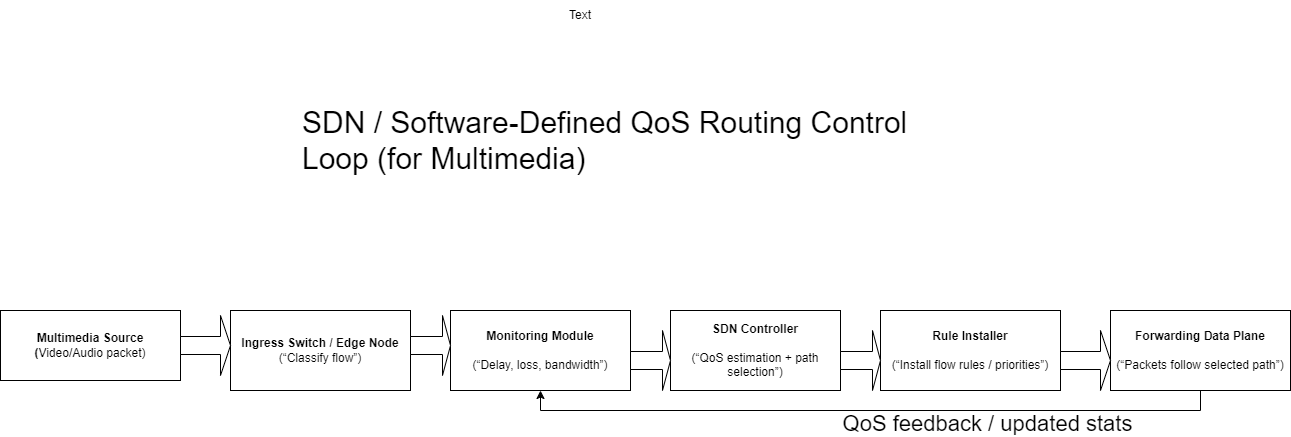
\includegraphics[width=1.00\textwidth]{fig_sdn_loop.png}
	\caption{Software-defined control loop for QoS-aware multimedia routing with monitoring and adaptive path selection (summary based on \cite{Suguna2022,9939088}).}
	\label{fig:sdn_qos_loop}
\end{figure}


	\section{Comparative Discussion}
    
When we discuss Quality of Service multimedia routing, we have to consider it. Quality of Service multimedia routing is not the same in all cases. What is best for Quality of Service multimedia routing in one location may not be best in another location.

It is also important to consider the impact of control overheads on the bandwidth for Quality of Service multimedia routing. To fully understand Quality of Service multimedia routing, we have to examine the impact of each method on the quality of the service, for Quality of Service multimedia routing that we can measure. Quality of Service aware multimedia routing is all about finding the path to accomplish things. It is about Quality of Service aware multimedia routing and how we can use it to accomplish things in the best possible manner. When we discuss Quality of Service multimedia routing, we are searching for the best path to take. Therefore, Quality of Service aware multimedia routing is the answer, to doing things the way.
	\subsection{Comparison criteria and classification logic}
    A similar comparison \cite{chen2020analysis} begins by establishing what “better” actually is for the multimedia transmission. The best metrics for comparison involve those that directly correlate to the user experience while also being feasible for the network. Delay and jitter relate to the interactivity and smooth flow of the multimedia content, while the loss rate relates to the visual artifacts or the audio dropouts. In addition to these metrics, the energy cost is important for sensor and IoT networks, and the control overhead is important for any wireless network that involves routing updates competing with multimedia content. It is also possible to divide the protocols into categories based on the decision-making process they use, whether they use a set of constraints or a scoring system, and whether they use local or global decision-making.
        \subsection{Multimedia QoS outcomes and tradeoffs}
        In most cases, designs that attempt to satisfy all of these goals at once do not actually achieve optimal performance in all of these areas. As a result, trade-offs between these goals can be very important. Designs that emphasize low end-to-end delay may take routes that are more prone to loss or instability. Designs that emphasize reliability, on the other hand, may take longer routes or maintain more routes, which can increase delay and consume additional bandwidth and power. If multiple metrics are used, the weights of these metrics can also have an impact. This is because small changes in weights can cause a protocol to shift between routes that emphasize stability and routes that emphasize raw throughput. In practice, this means that a protocol can be considered successful in that it improves one of these metrics, but still fails to provide a good experience for the user because of increased variability or additional buffer times. The only way to really understand the performance of a QoS protocol is to look at all of these metrics together, rather than in isolation.
        \subsection{Overhead, scalability, and responsiveness under dynamics}
        However, routing intelligence is not free. The use of "collecting link metrics, bandwidth probing, and reporting" of some of the protocols can result in a decrease of bandwidth availability for multimedia packets. When mobility is considered, the quick response of the protocols can be an advantage for ensuring accurate routes. However, this can also result in route oscillations, where the routes change too frequently, causing the packets to get reordered, with some of them being lost. When dense contention is considered, the noise can result in unstable decisions, especially if the quick response of the protocol is considered. It is also important to evaluate the scalability of the protocol, i.e., whether the decisions are being taken locally with limited neighborhood information or whether the protocol has global information of the network state, which can be expensive. It is also important to evaluate the performance of the protocol not only by comparing the steady-state performance of the protocol with other protocols, but also by comparing the graceful response of the protocol to changes such as handoffs, congestion buildup, and link failures.
        \subsection{Practical implementability and evaluation realism}
        A final dimension concerns how readily a routing approach can be implemented and assessed with realistic assumptions. Some protocols may rely on cross-layer information, good bandwidth estimation, or synchronized knowledge of the channels. These may be difficult to obtain on real devices. Other protocols may assume stable traffic patterns or simple interference models that are not realistic in a busy wireless network. While the simulation results may be promising, the viability of a protocol depends on whether it can be implemented on the platform with sufficient resources to perform all required measurements, processing, and signaling. A discussion of the various techniques with an emphasis on implementability will reveal which techniques are robust to information uncertainty, which techniques are robust to measurement delays, and which techniques are robust to violations of assumptions.

	\section{Practical Insights and Use Cases}
    Routing aware of QoS becomes most useful when related to tangible multimedia-driven applications where loss of service can be traced in real-time by the end user. Practical implementations frequently have real-time constraints on latency and reliability, continuous sensing, and tremendously limited devices, which are not able to support a high level of control overhead. One example use case is Wireless Body Sensor Networks, which tend to combine sensitive physiological measurements with real-time constraints and very high energy constraints and often work in a world whose connection characteristics vary with posture, motion and shadowing of the body. Under these conditions, QoS-aware routing should also adhere to various constraints, namely, timeliness, reliability, and power consumption, and ensure a stable communication near the human organism. These operational constraints drive the multi-constraint routing design that clearly considers QoS as a demand but not a best-effort result.




    \subsection{Continuous health monitoring with mixed data streams}
    It is possible \cite{zuhra2020miqos}for a variety of different kinds of traffic patterns to be generated by the wearable or implantable sensor devices, which can be similar to the multimedia data streams. However, the major concern is that any additional delay or loss of packets will make the process completely ineffective for applications such as the near-real-time interpretation process, etc. The QoS routing can be extremely critical for these applications, as it is possible for the reliability of the data delivery to be ensured and the delay to be controlled regardless of the changing conditions due to the movement of the patient. This routing is extremely practical as it is possible for the routing to be dependent on the relevance of the data being sent, with some of the data having more stringent requirements.
    \subsection{Motion and activity scenarios with high variability}
    Scenarios such as rehabilitation, sports monitoring, and ambulatory patient tracking involve fast changes in posture and high variations in link quality. In such cases, the routing protocols are likely to fail because the links may not remain stable over time; they may be good one minute and bad the next, depending upon the orientation of the body or the movement of the limbs or even temporary obstructions. Realistic QoS-aware routing protocols should exhibit stable performance in the presence of such changes and should not make decisions that could result in high jitter bursts or transient failures. A realistic routing protocol should adapt quickly without using high signaling because rebuilding routes frequently may not only consume power but also disrupt the packet delivery process.
    \subsection{Safety-critical alerts and reliability-focused delivery}
    There are also applications related to body networks with thresholds and abnormality detection, in which delayed or lost packets may diminish the value of the alarm generated. Even if the data rate is not extremely high, the service requirement is stringent because the value of the alarm is time-sensitive. A feasible design for QoS-aware routing in such an environment focuses on the minimization of the probability of missing or delayed critical packets, and it may be necessary to balance both reliability and delay rather than trying to optimize one metric over the other. This example also shows that the performance of QoS-aware routing cannot be measured using average metrics because the traffic related to safety applications is severely impacted by the worst case in delay and loss.
	\subsection{ntegration with personal gateways and edge connectivity}
    In practice, body sensors will typically communicate via a personal gateway, which will then transmit data to an edge server/cloud for visualization/analysis. The routing mechanism within the body network has to be adapted to the capabilities of the gateway, which has constrained power sources, changing radio conditions, and other background traffic competing for bandwidth on the gateway device. The aim of QoS-aware routing in practice is to manage the stability of the intra-body network so that the action of the gateway can be effective. This is because the quality of a real-time monitoring service is dependent on this end-to-end quality.

	\section{Challenges and Open Issues}
    The issue \cite{Promkotwong2007QMRP}of sustaining the Quality of Service, which is needed to support the routing of multimedia information in the wireless networks, is considered as one of the most significant issues in this sphere, taking into account the necessity to transfer time-bound information regarding the media across a net which is affected by sudden limitations simultaneously. The multimedia routing is defined by massive volumes of the traffic bearing in mind that the transmission of the media should be conducted continuously. As such, any slight variation on signal quality is seen to have serious impacts on the quality of the media. Conversely, the majority of the wireless multimedia services are seen to lack adequate control signals keeping in mind the fact that there is a need of rescalculating routes keeping the limited quantity of bandwidth and energy used in supporting the media stream. Thus, the challenge ceases to be identified as the identification of routes with good QoS, but their maintenance without creating network instability. The problems encountered in the discipline are no longer on the routes with good QoS, but on the paths that are scalable, taking the dynamics of the network into consideration.
	\subsection{Mobility, interference, and unstable link quality}
    Wireless multimedia \cite{Singal2022} routes have to cope with the fast changes in the qualities of the links due to the effects of mobility, multipath fading, and changes in interference. This implies that routes may fail abruptly, and the routes have to be repaired, which may lead to bursts of delay, loss, and reordering, which can be very detrimental to video and interactive audio. In addition, the presence of interference and contention complicates the prediction of the route qualities since the route may have a very good physical layer quality, while the service provided by the route may be poor due to the presence of other neighboring transmissions that may lead to collisions and/or backoff delays. This implies that it may be hard to obtain a stable jitter and bounded delay, especially in dense networks and the presence of competing multimedia routes. An important open problem is how to utilize the measurement information that is available and sufficient to drive the routing decisions without reacting too strongly to the short-term changes in the qualities of the links.
    \subsection{Multicast and group communication complexity}
    There are also many multimedia applications that require one-to-many communication, such as video sharing, situational awareness, and communication in a group. The mesh multicast protocol may also improve the reliability of the communication system, but it also makes the system more complicated because the protocol should maintain the forwarding state towards the receivers and also deal with the changes in the group without incurring high overhead. In the edge ad hoc networks, the group may frequently change, and the receivers may require different qualities of service, making it difficult to determine the ‘best’ multicast structure because it would be difficult to meet the minimum QoS requirements with the performance variations due to the contention and hidden terminal effects in the network.
    \subsection{Control overhead, scalability, and resource limits}
	The QoS-aware routing often relies on the collection and distribution of certain states, such as link delay estimates, congestion levels, or available bandwidth. In wireless networks, this kind of traffic directly competes with the multimedia traffic. Excessive monitoring traffic can degrade the throughput and increase the end-to-end delay. Therefore, the QoS-aware routing in wireless networks becomes challenging. The issue of scalability arises as the network size increases. In such scenarios, the maintenance of global or near-global states becomes impractical. Even in the case of a decentralized multicast routing scheme, excessive changes in the topology can cause significant overhead in updating the mesh. The challenge here is to devise mechanisms to reduce the signaling while retaining the advantages of QoS-aware routing.
    \subsection{Heterogeneity and fairness under mixed traffic loads}
    In the real world, there are not just one or two types of traffic; there are multimedia traffic, there are control messages, there are sensor updates, there are best-effort data packets, and so on. If you try to lock in the quality of service for multimedia traffic, you can starve other traffic flows, which defeats the notion of fairness. If the isolation between different types of traffic is weak, then the non-multimedia traffic can overwhelm the gains of the multimedia traffic.



In the context of edge ad hoc networks, there are different devices that are connected together, and these devices have different capabilities, different transmission ranges, different energy levels, and so on. This can create an uneven forwarding load across the devices. Some devices can end up forwarding traffic for other devices, and if we are using multicast, then these devices can end up forwarding traffic for multiple devices.



There are open issues that are still not clear on how we can allocate the resources fairly across the different flows, how we can allocate the workload fairly across the different devices, and how we can create multicast forwarding that meets the quality of service requirements while keeping the network sustainable over the long term.
	\section{Future Directions}
    It is expected that future research in QoS-aware routing protocols for multimedia communication will focus on developing routing paradigms that are capable of reasoning in an uncertain world, are able to quickly adapt to the dynamic wireless world, and make routing decisions based on user experience quality, as opposed to traditional network-centric quality of service measures. With the increasing importance of multimedia communication in dense IoT, mobile, edge, and other environments, as well as sensing environments with limited resources, routing protocols are expected to satisfy different requirements, including low latency, high reliability, low energy consumption, and minimal control overhead. The primary focus of future research in routing protocols is expected to be the transition from traditional fixed, hand-designed routing paradigms to routing paradigms that are able to learn the optimal strategy from observations of the behavior of the networks, while being lightweight and interpretable. This is clearly demonstrated in the work on swarm intelligence-based routing protocols, which considers routing optimization with multiple sets of constraints.
    \subsection{Learning-assisted and adaptive optimization for dynamic QoS}
    A promising approach is to make QoS-based routing \cite{Benmansour2021} more adaptive by using learning and optimization together. Rather than using static weights for metrics such as delay, jitter, loss, and energy, a QoS-based routing system can change its policy for making routing decisions as the environment changes, e.g., due to increased mobility, increased contention, or bursty traffic. Hybrid approaches can be used to combine light-weight prediction of link qualities and metaheuristic optimization to avoid poor local optima and to react to changes when the system moves to a new operating regime. The main difficulty is to keep the learning and optimization processes low enough in complexity for wireless sensor and IoT networks while avoiding the problem of route instabilities due to excessive route changes.
    \subsection{QoE-driven routing for multimedia perception}
    Another avenue is to more directly relate routing objectives to Multimedia Quality of Experience. While QoS parameters are important, they do not always correlate to what is actually perceived by users, especially when considering how codec, buffering, and error concealment mechanisms can affect certain types of network issues more than others. QoE-based routing is an approach to more directly relate user-perceived quality to routing decisions that take into account which factors have the greatest impact given a particular scenario. The optimization-based routing approaches provide support for this avenue of research because of their flexibility to modify the optimization function. 
    \subsection{Energy-aware intelligence and sustainable routing control}
	
The cost of multimedia transmission can also be high in battery-powered nodes, especially in cases where large packets, retransmission, and control signaling consume power. The future routing schemes will have to consider energy consumption, not just as a secondary metric but rather as a primary metric, along with other metrics such as delay and reliability. The swarm intelligence-based routing schemes seem promising in addressing these issues by delegating the responsibility of routing to all nodes in the network, ensuring that the traffic is distributed appropriately, preventing the selection of the same nodes for routing, and ensuring the overall lifetime of the network without compromising the quality of service of the multimedia traffic. The question is how to achieve all these without increasing the complexity of the routing algorithm.
\subsection{Standardized benchmarking and reproducible evaluation}
One way forward is to improve our ability to evaluate QoS routing so that results from different approaches may be compared and reproduced. As the results of QoS routing protocols in the multimedia environment depend considerably on the underlying mobility model, interference scenarios, traffic patterns, and application-level behavior, a particular protocol may not necessarily perform well in another scenario. Advancements will come from the development of common practices in benchmarking and scenario descriptions to enable researchers to better determine which ideas will prove robust and which are merely specific to the particular environment in which they were developed. Reproducibility will also be important in optimization-based QoS routing as the performance of such algorithms may depend on how it’s initialized, how long it runs, and when it stops.
	\section{Conclusion}
	QoS-aware routing is considered to be one of the most important factors that play a crucial role in facilitating a reliable multimedia communication in wireless networks, particularly considering that it is an undeniable fact that video communication and other forms of multimedia communication are highly sensitive to factors such as delay, jitter, packet loss, and bandwidth changes. As already indicated by the methods discussed within this report, it is important to understand that the best way to improve the overall performance of multimedia communication is to ensure that the routing protocol is made aware of a number of factors, rather than relying on the protocol to follow the shortest path to the final destination. The utilization of metric-based routing allows a straightforward relationship to be made between the needs and the routing process. The utilization of a multipath routing protocol enhances the reliability of the communication process considering that the link may be unstable at any given time. The optimization-based methods improve the search space to ensure a better balance between QoS and availability. The utilization of a multi-layer approach or software-defined networking enhances the accuracy of the process.
    Meanwhile, no single method provides universal guarantees in the face of mobility, interference, and contention, especially when control costs and energy are critical. Ultimately, the choice of method depends on the application scenario, e.g., smart city IoT sensor networks, MANET video transmission, edge multicasting, or body sensor networks. The most promising way forward is clearly towards adaptive, QoE-aware, and scalable routing schemes that can provide continuous quality of service within multimedia applications, yet are implementable in wireless devices.
	

	\bibliographystyle{plain}
	\bibliography{references}
	
\end{document}
